\documentclass[a4paper]{article}
% Margins
\usepackage{a4wide}
% Write dutch
\usepackage[dutch]{babel}
% Used for images
\usepackage{graphicx}
\usepackage{epstopdf}
% Needed to use headers
\usepackage{fancyhdr}
% Used for the euro symbol
\usepackage[gen]{eurosym}
% Used for optimal usage of gensymb
\usepackage{textcomp}
% Used for the degree symbol
\usepackage{gensymb}
% Used for captions and subcaptions on images
\usepackage{caption}
\usepackage{subcaption}
% Used for tables
\usepackage{tabu}
% Used for colors
\usepackage[usenames,dvipsnames,svgnames]{xcolor}
\usepackage{caption}
\usepackage{minted}
\usemintedstyle{colorful}
% No tab at start of paragraph
\setlength{\parindent}{0em}
\setlength{\parskip}{1em}
% Allows to change margin for a block
\def\changemargin#1#2{\list{}{\rightmargin#2\leftmargin#1}\item[]}
\let\endchangemargin=\endlist 
% Header
\pagestyle{fancy}
\fancyhf{}
\renewcommand{\headrulewidth}{0pt}
\fancyhead[HR]{\thepage}
\fancyhead[L]{Titouan Vervack}
\begin{document}
\begin{titlepage}
\fontsize{12pt}{14pt}\selectfont

\begin{center}

% Het logo van de Universiteit Gent
\includegraphics[height=3cm]{logo}

\vspace{1cm}

\fontsize{14pt}{17pt}\selectfont
% De Faculteit:
\textsc{Master of Science in Computer Science Engineering}
\fontsize{12pt}{14pt}\selectfont
\vspace{0.3cm}

\vspace{1.2cm}

Academic year 2015--2016

\vspace{2.8cm}

\fontsize{17.28pt}{21pt}\selectfont

% De titel van de thesis:
\textsc{Project Queueing Analysis and Simulation}
\fontsize{14.28pt}{21pt}\selectfont
\textsc{Discrete Event Simulator}

\fontseries{m}
\fontsize{12pt}{14pt}\selectfont

\vspace{2.8cm}

% De auteur van de thesis:
Titouan Vervack

\end{center}
\end{titlepage}
\newpage
\fontsize{12pt}{16pt}\selectfont

\section{Performance measurements}
In this section the observed performance measurements using the FCFS, LCFS, SSTF, and ROS scheduling disciplines are discussed. The performance measurements that have been observed are queue content, waiting time and sojourn time. The confidence interval and sample means variance, produced through the batch means method, for the estimated queue content are also shown.
All of the code, written for this project, can be found in \ref{sec:code}.

It is important to note that for we observe at random times. This has been achieved by scheduling monitor events, which do not change the state of the system, at times sampled from a Poisson distributions, because of the PASTA property we know that these times can be considered random. The same names as in the code of course notes are used. aA is the $\alpha$ of the arrivals, bA the $\beta$, aS is the $\alpha$ of the services, $bS$ is the $\beta$ of the services and c is the number of servers. If the $\alpha$'s and $\beta$'s are not mentioned, they are presumed to be 1 for the arrivals and 1 for the services. If the number of servers is not mentioned, it is presumed to be 1. Lastly, the $\lambda$ for the Poisson process monitoring the system is $\frac{aS + bS + aA + bA}{3}$.

\subsection{Queue content}
For the queue content with our default values, we see that in every case, but the SSTF, the queue content is quite high most of the time. This is because we are drawing service rates and arrival rates from the same distribution. Sometimes the arrivals will be a little faster than the the services, hence the down drafts, on the other hand they will also be be longer at some times, causing the peaks. The queue content of SSTF is lower overall, because it first gets rid of all the services that can be done quickly. However at some time it will run out of service that can be done quickly and it the content will rise momentarily. If we now increase our $\beta$ of the services and see that our queue content bounces between 0 and 10, this is because services now take less long than arrivals.
\begin{figure}[H]
\begin{subfigure}{.5\textwidth}
  \centering
  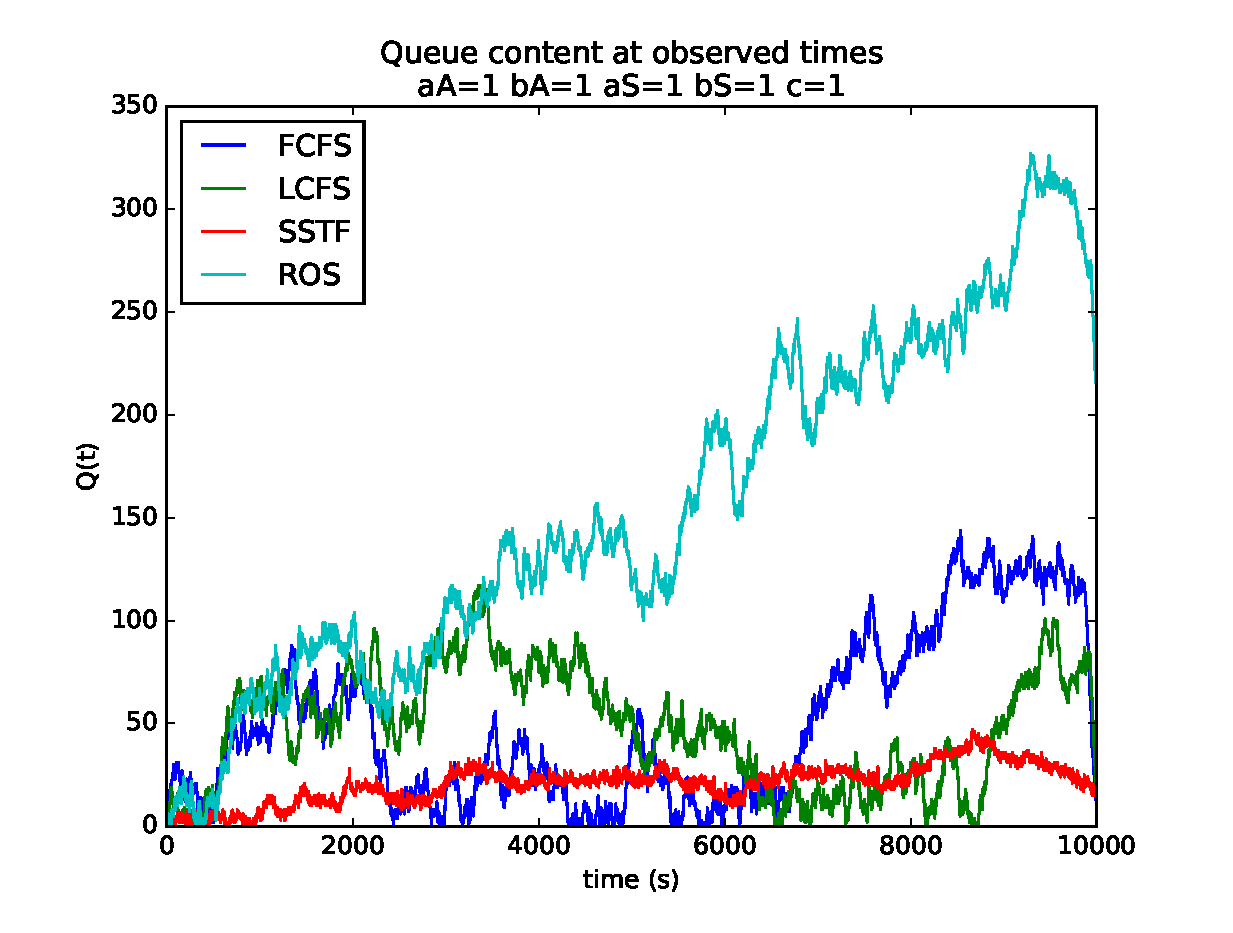
\includegraphics[width=\linewidth]{../figures/queue_content11111}
  \label{fig:qc}
\end{subfigure}
\begin{subfigure}{.5\textwidth}
  \centering
  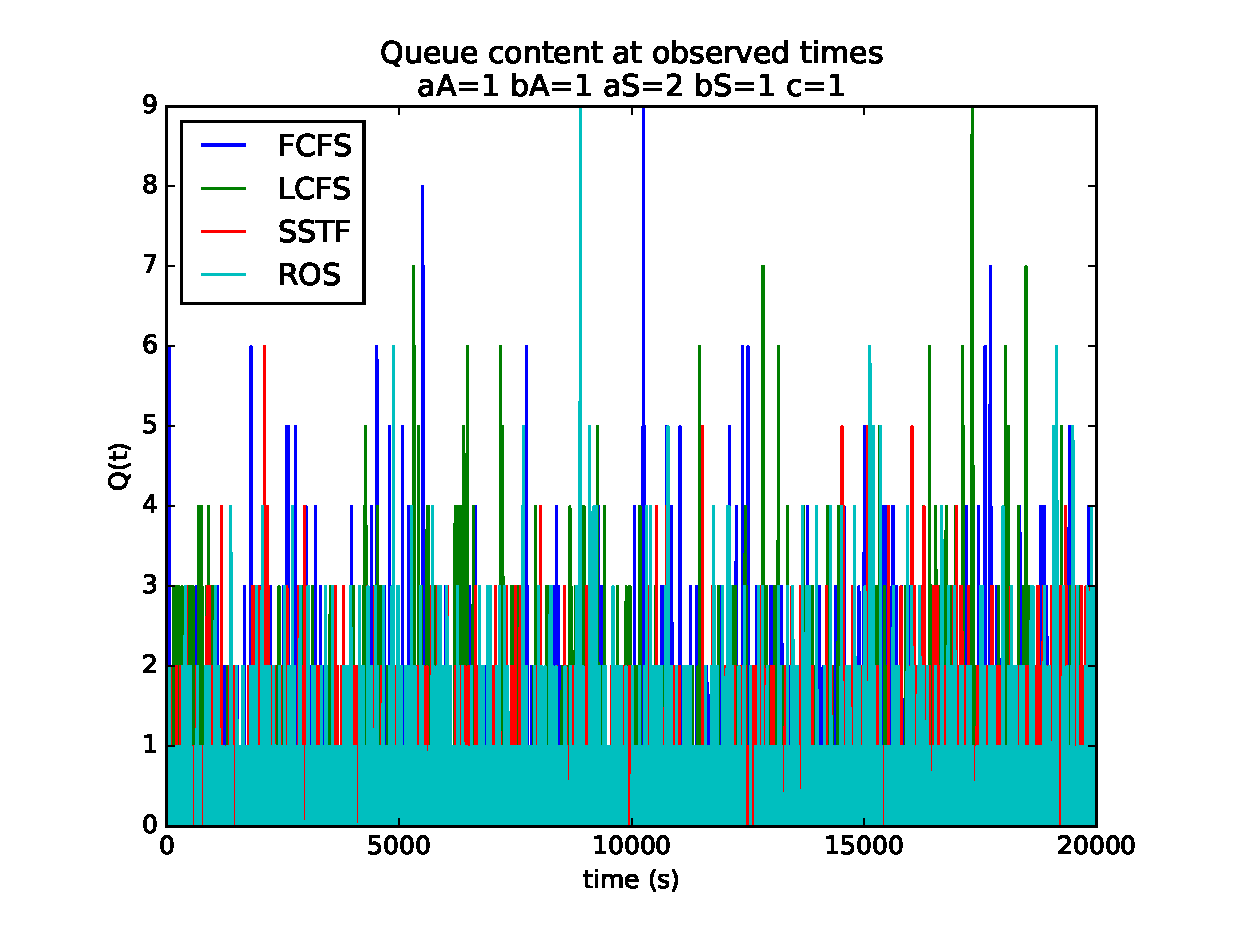
\includegraphics[width=\linewidth]{../figures/queue_content11211}
  \label{fig:qca}
\end{subfigure}
\end{figure}

If we increase  $\alpha and \beta$ of our arrival process, the arrivals will be faster than the services and thus we see the queue content rising until the maximum amount of arrivals has happened after which we see a steady decrease of the customers. SSTF performs better in this case for the same reasons as mentioned before. Adding more servers to allows everything but FCFS to cope with the number of arrivals.
Checking out LCFS, we notice that the peak of the distribution is around 2000, but since FCFS first has to has process all of the others, it will only notice this maximum later on, at about 4000s.
\begin{figure}[H]
\begin{subfigure}{.5\textwidth}
  \centering
  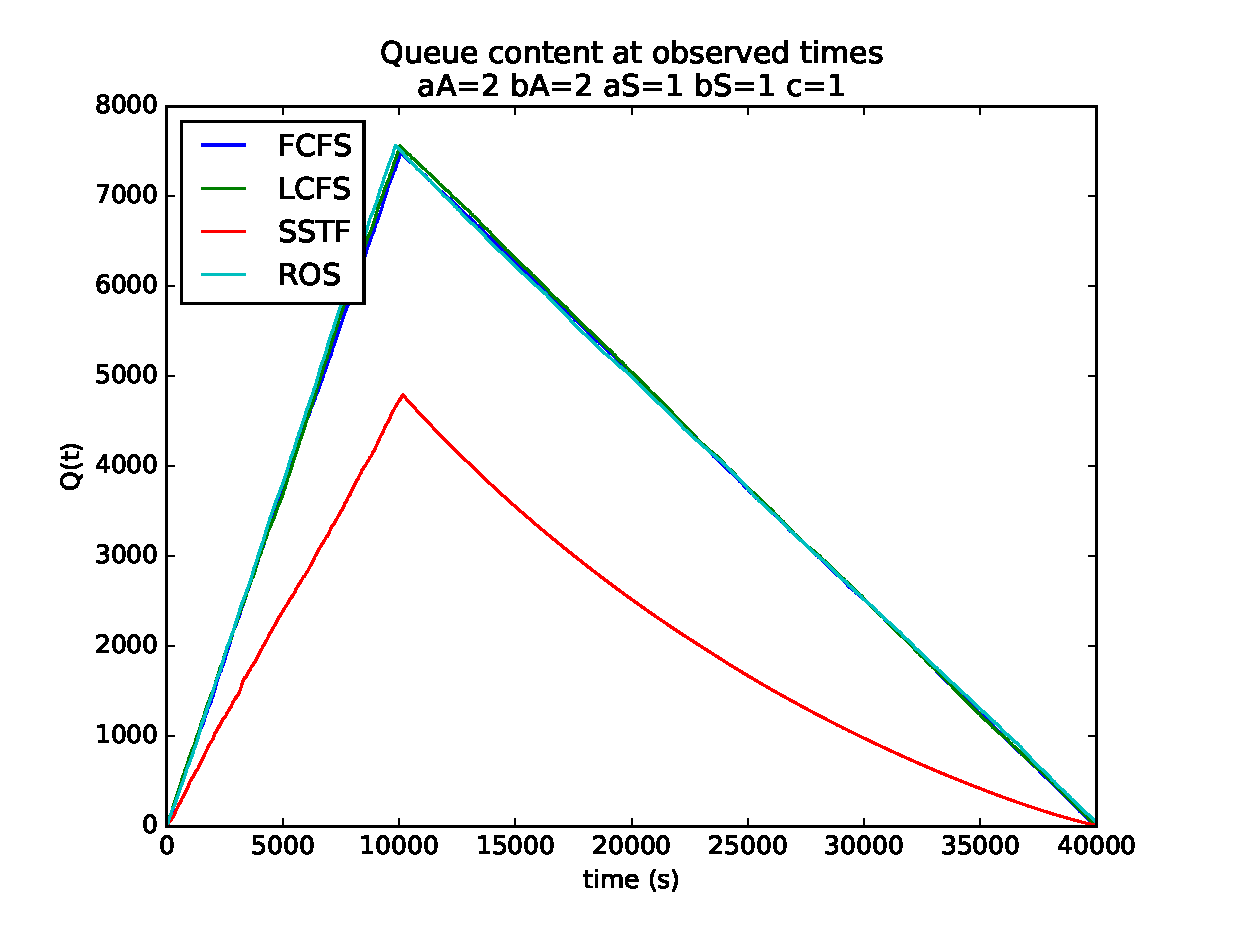
\includegraphics[width=\linewidth]{../figures/queue_content22111}
  \label{fig:qcaa}
\end{subfigure}
\begin{subfigure}{.5\textwidth}
  \centering
  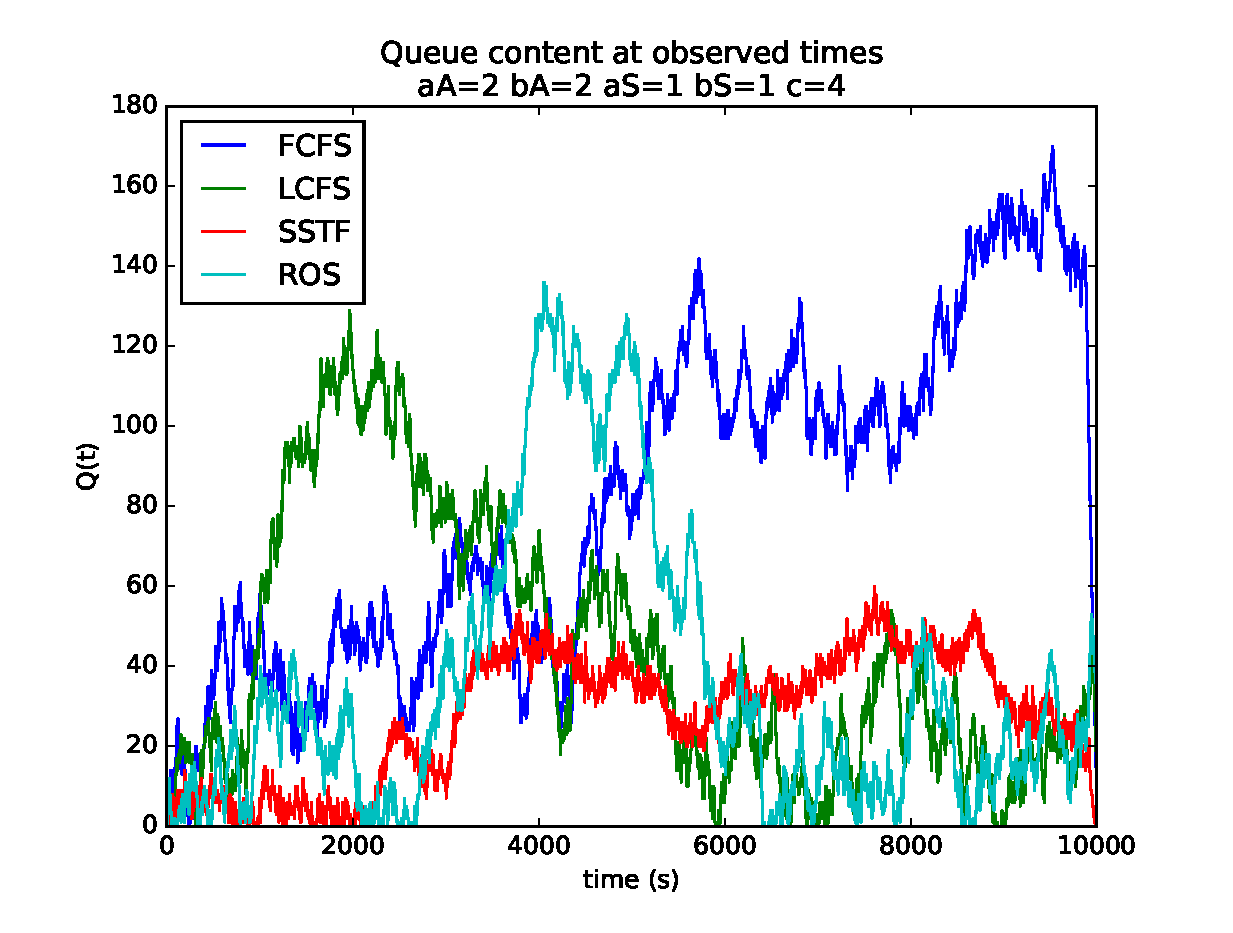
\includegraphics[width=\linewidth]{../figures/queue_content22114}
  \label{fig:qcaaa}
\end{subfigure}
\end{figure}

\subsection{Waiting time}
With our default values, waiting times converge after some time, however for ROS they go to infinity.
When we increase the server count the waiting time converges to zero because we now have two servers while the arrival and service rate are nearly the same. Increasing the $\beta$ of the services causes the services to happen faster than the arrivals, which causes the waiting time to converge to 0. Again we see, when we increase $\alpha$ and $\beta$ of the arrivals, our waiting times goes to infinity because arrivals are now faster than services and we can not cope with it.
\begin{figure}[H]
\begin{subfigure}{.5\textwidth}
  \centering
  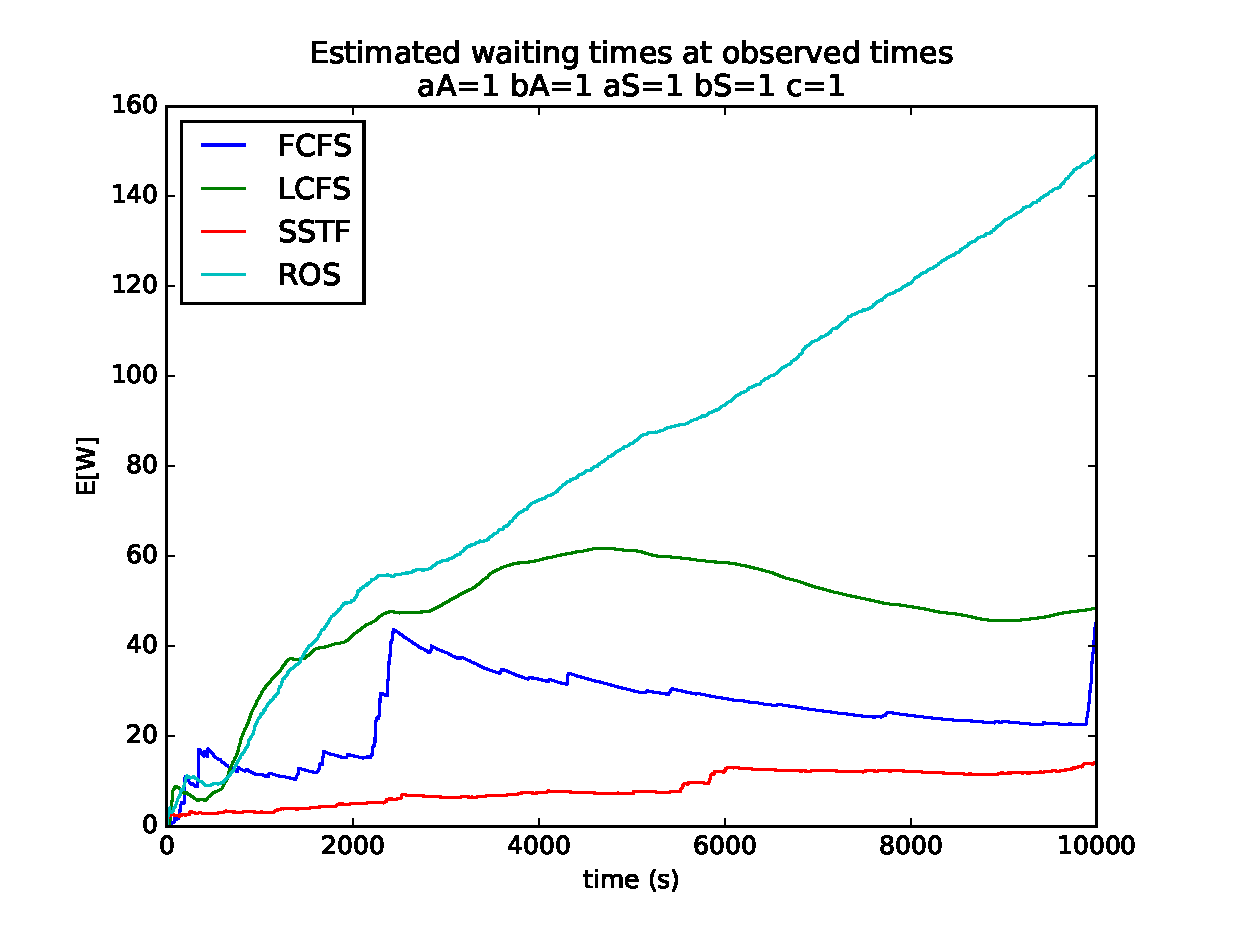
\includegraphics[width=\linewidth]{../figures/waiting_times11111}
  \label{fig:wt}
\end{subfigure}
\begin{subfigure}{.5\textwidth}
  \centering
  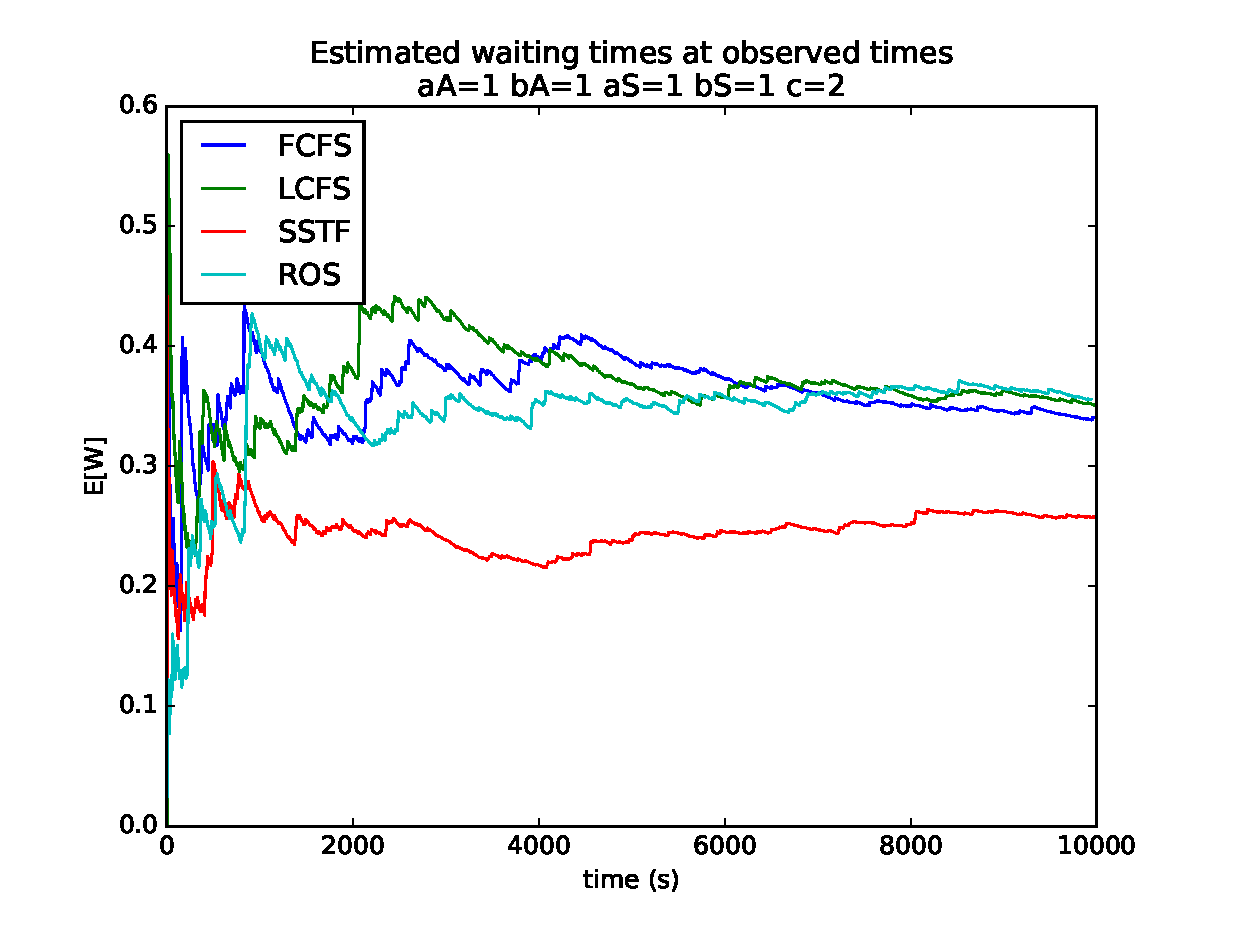
\includegraphics[width=\linewidth]{../figures/waiting_times11112}
  \label{fig:wta}
\end{subfigure}
\end{figure}

\begin{figure}[H]
\begin{subfigure}{.5\textwidth}
  \centering
  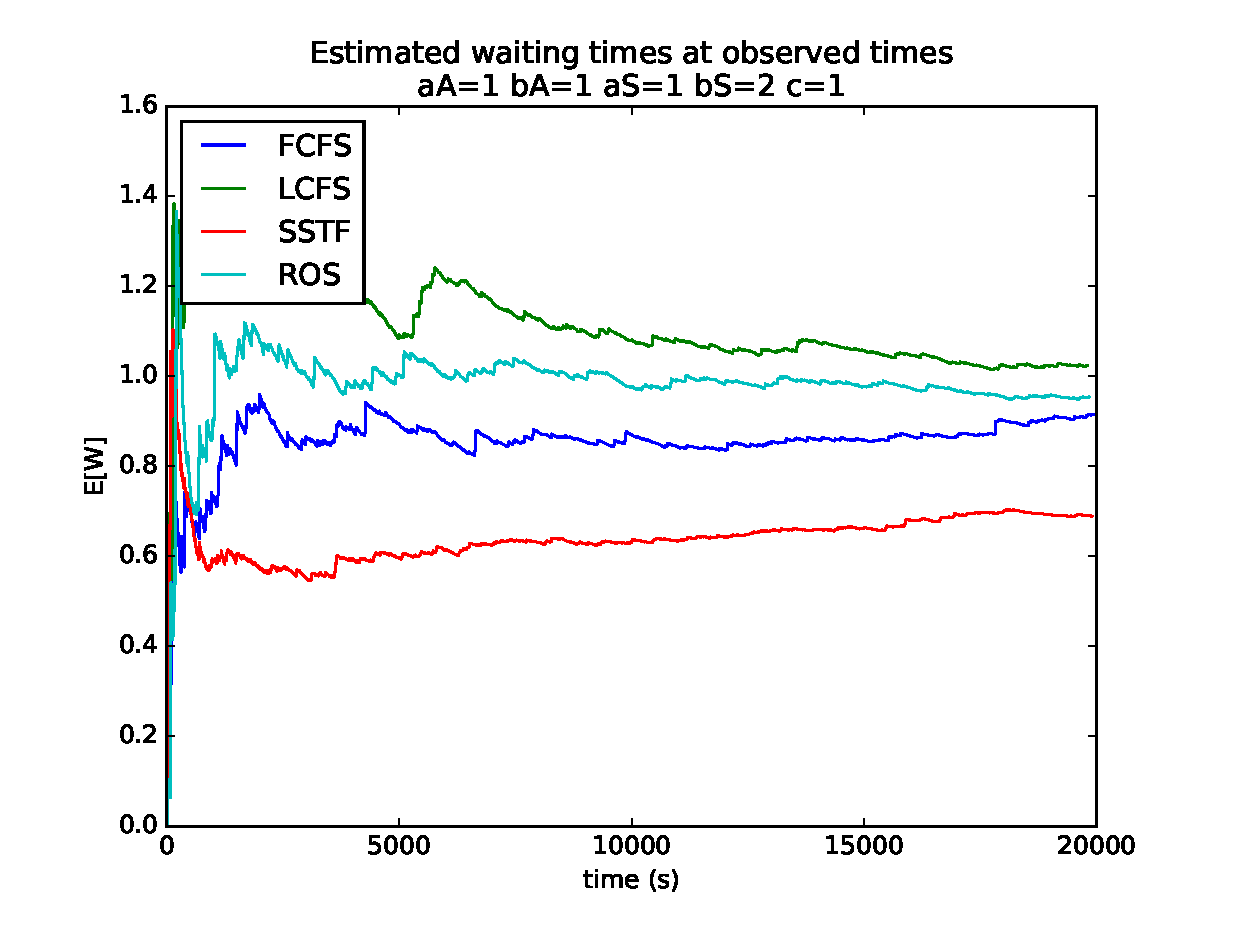
\includegraphics[width=\linewidth]{../figures/waiting_times11121}
  \label{fig:wtaa}
\end{subfigure}
\begin{subfigure}{.5\textwidth}
  \centering
  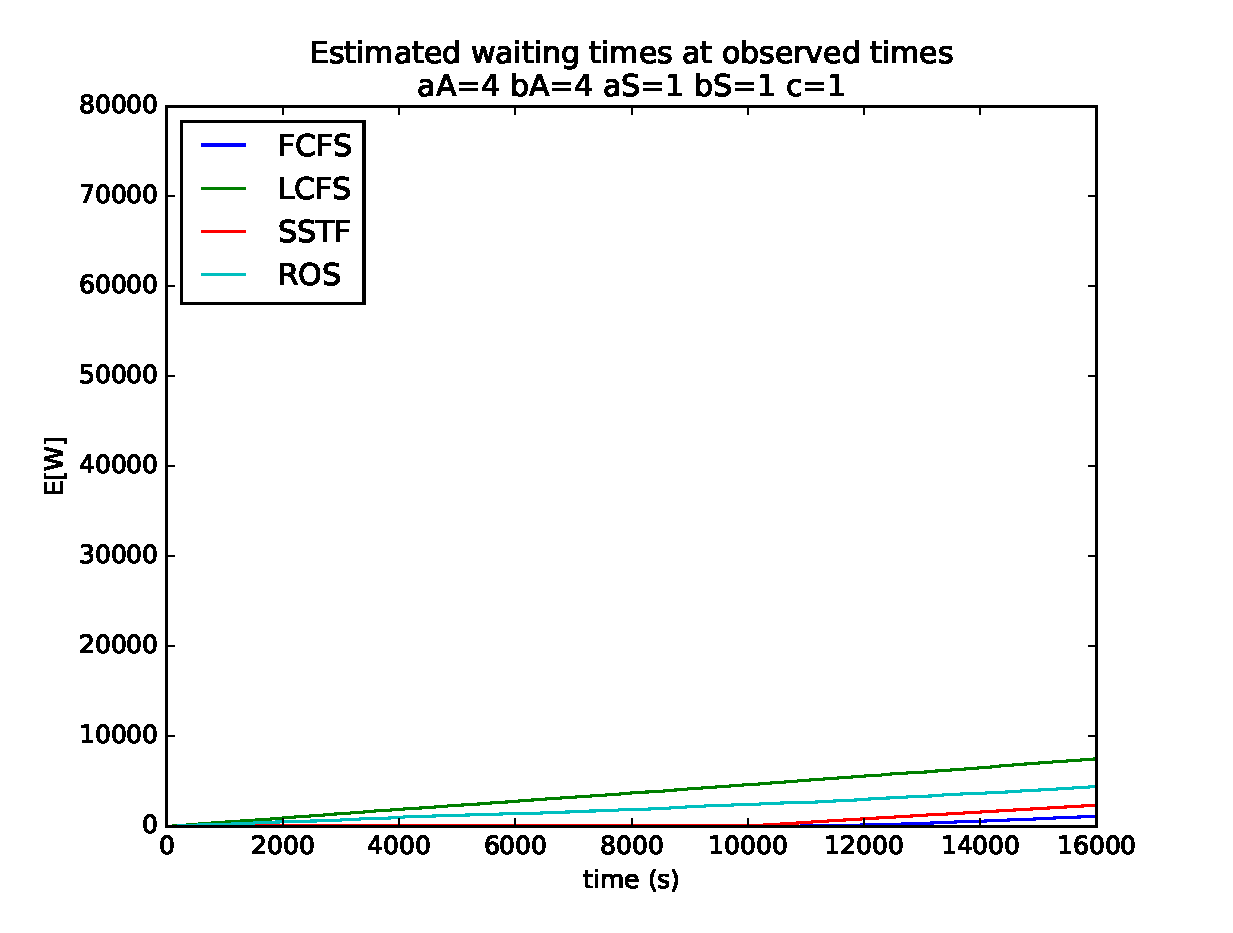
\includegraphics[width=\linewidth]{../figures/waiting_times44111}
  \label{fig:wtaaa}
\end{subfigure}
\end{figure}
\subsection{Sojourn time}
The sojourn time remains almost identical to the waiting time as it is the waiting time + the service time. The sojourn time can thus only be significantly different if the service time takes up the majority of the sojourn time. Having a longer service time however, causes a longer waiting time, thus it can never make a significant difference. We just show two graphs from waiting time again to show that there is indeed almost no difference.
\begin{figure}[H]
\begin{subfigure}{.5\textwidth}
  \centering
  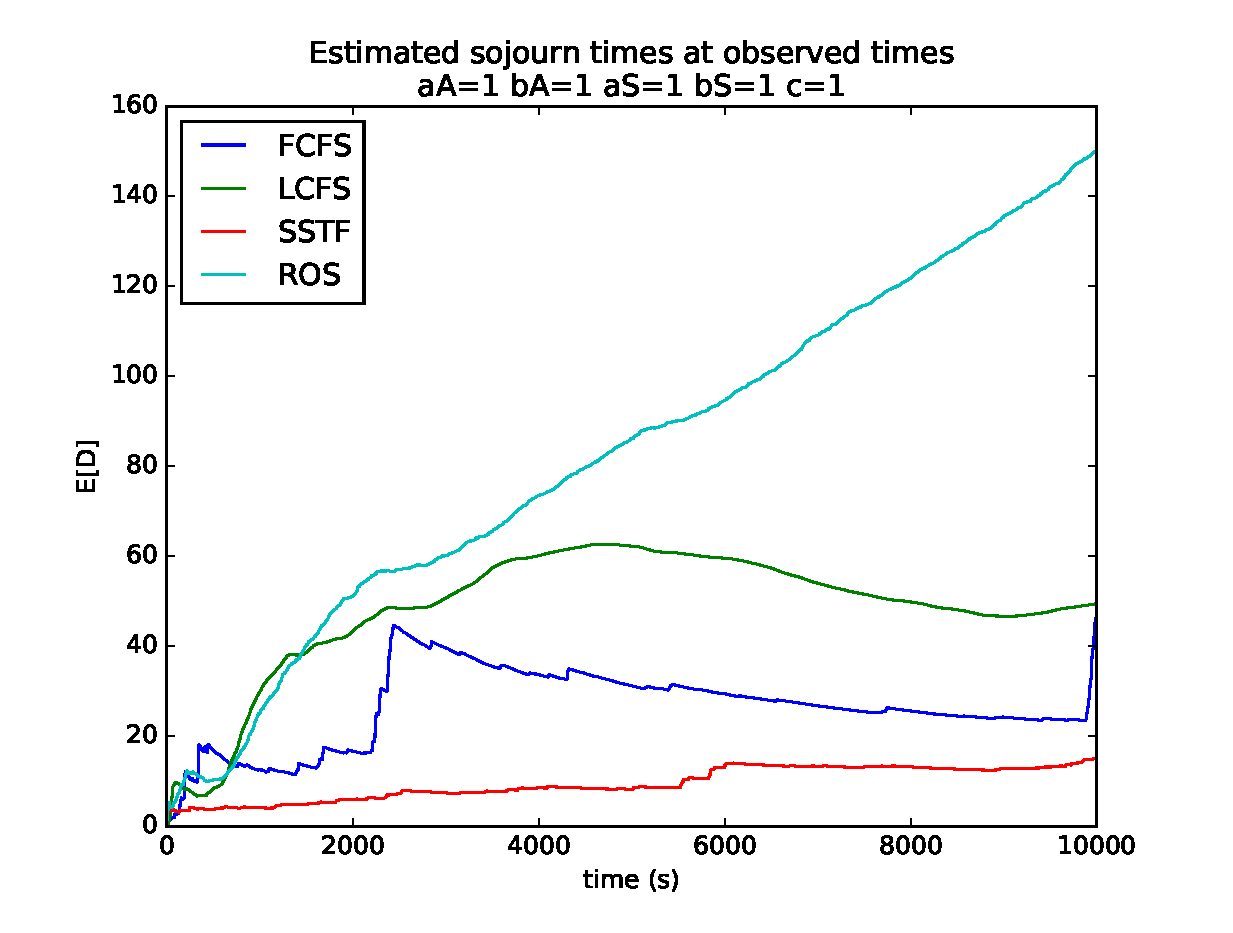
\includegraphics[width=\linewidth]{../figures/sojourn_times11111}
  \label{fig:st}
\end{subfigure}
\begin{subfigure}{.5\textwidth}
  \centering
  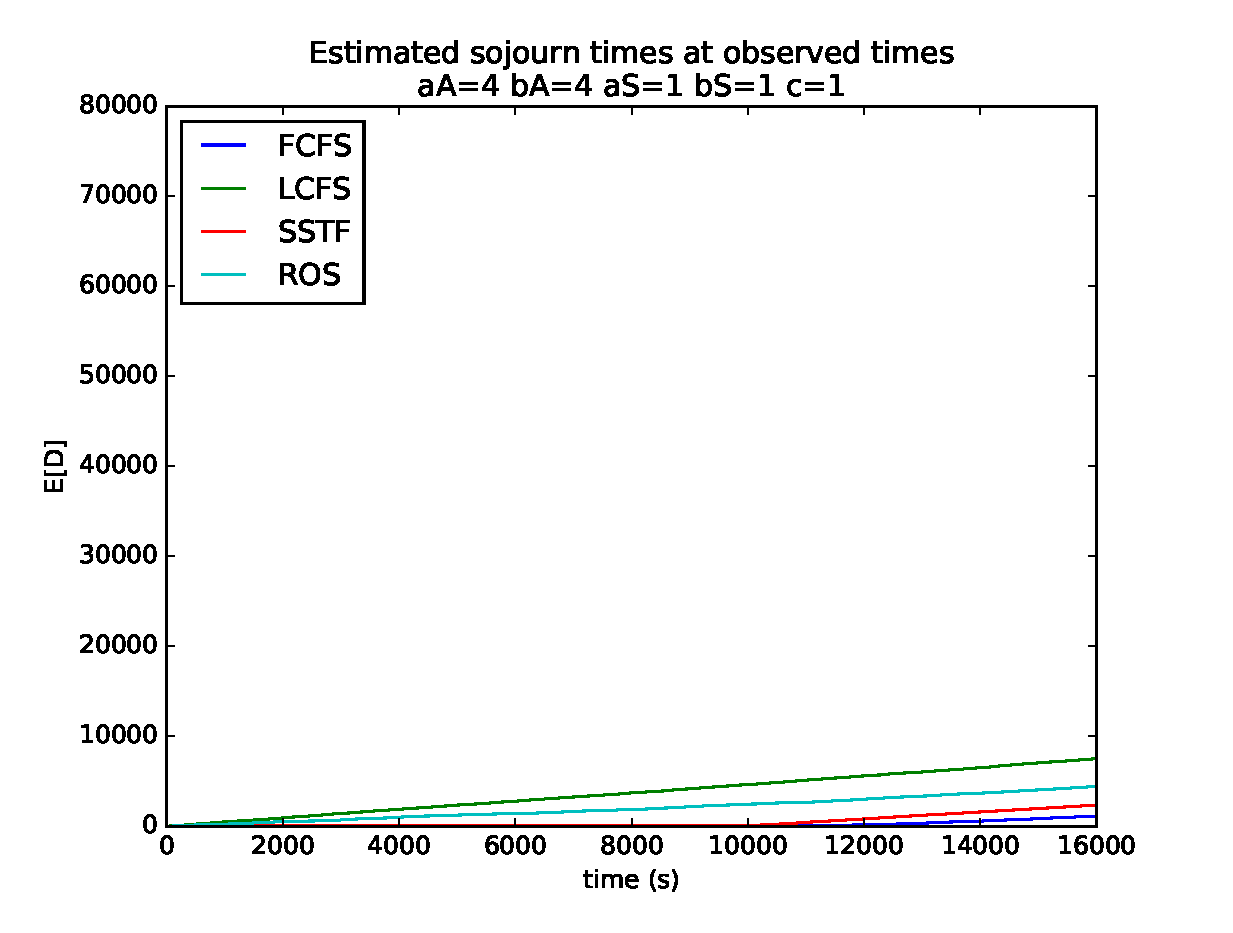
\includegraphics[width=\linewidth]{../figures/sojourn_times44111}
  \label{fig:sta}
\end{subfigure}
\end{figure}
\subsection{Batch means method}
For the batch means method a $k_{p}$ of $2.58$ was chosen, this value can be found in the standard normal distribution tables (Z-tables). It is the factor needed to calculate the 99\% confidence interval.

The plots for the different scheduling disciplines have been not been shown in one figure as before, as it would make the figure very unclear.
The below figures depict the 99\% confidence interval for the estimated waiting time obtained through the batch means method.
\begin{figure}[H]
\begin{subfigure}{.5\textwidth}
  \centering
  \includegraphics[width=\linewidth]{../figures/FCFS_batch_mean_ci}
  \label{fig:fcfsbm}
\end{subfigure}%
\begin{subfigure}{.5\textwidth}
  \centering
  \includegraphics[width=\linewidth]{../figures/LCFS_batch_mean_ci}
  \label{fig:lcfsbm}
\end{subfigure}
\end{figure}

\begin{figure}[H]
\begin{subfigure}{.5\textwidth}
  \centering
  \includegraphics[width=\linewidth]{../figures/SSTF_batch_mean_ci}
  \label{fig:sstfbm}
\end{subfigure}%
\begin{subfigure}{.5\textwidth}
  \centering
  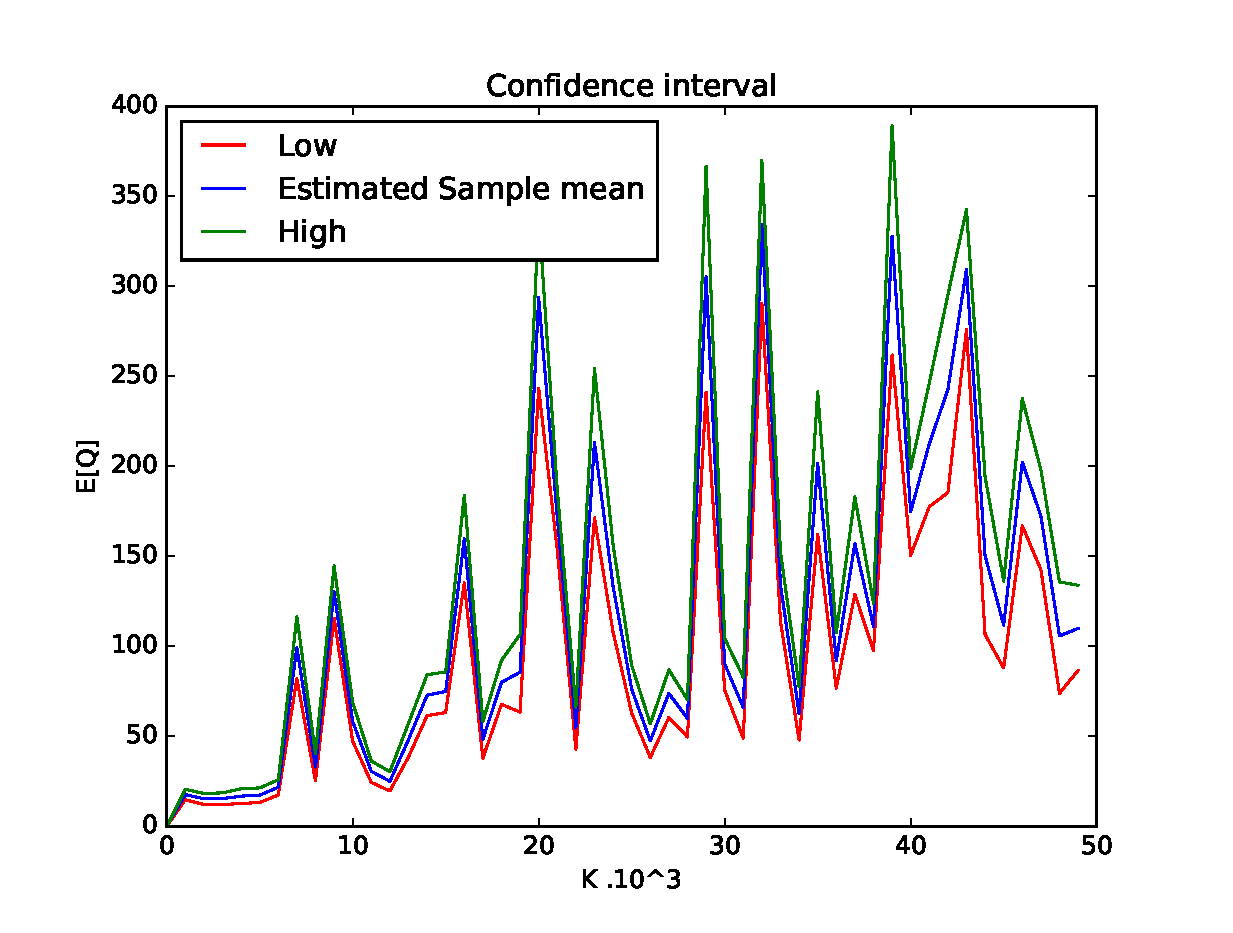
\includegraphics[width=\linewidth]{../figures/ROS_batch_mean_ci}
  \label{fig:rosbm}
\end{subfigure}
\end{figure}

Below you can find the sample variances obtained through the batch means method.
\begin{figure}[H]
  \centering
  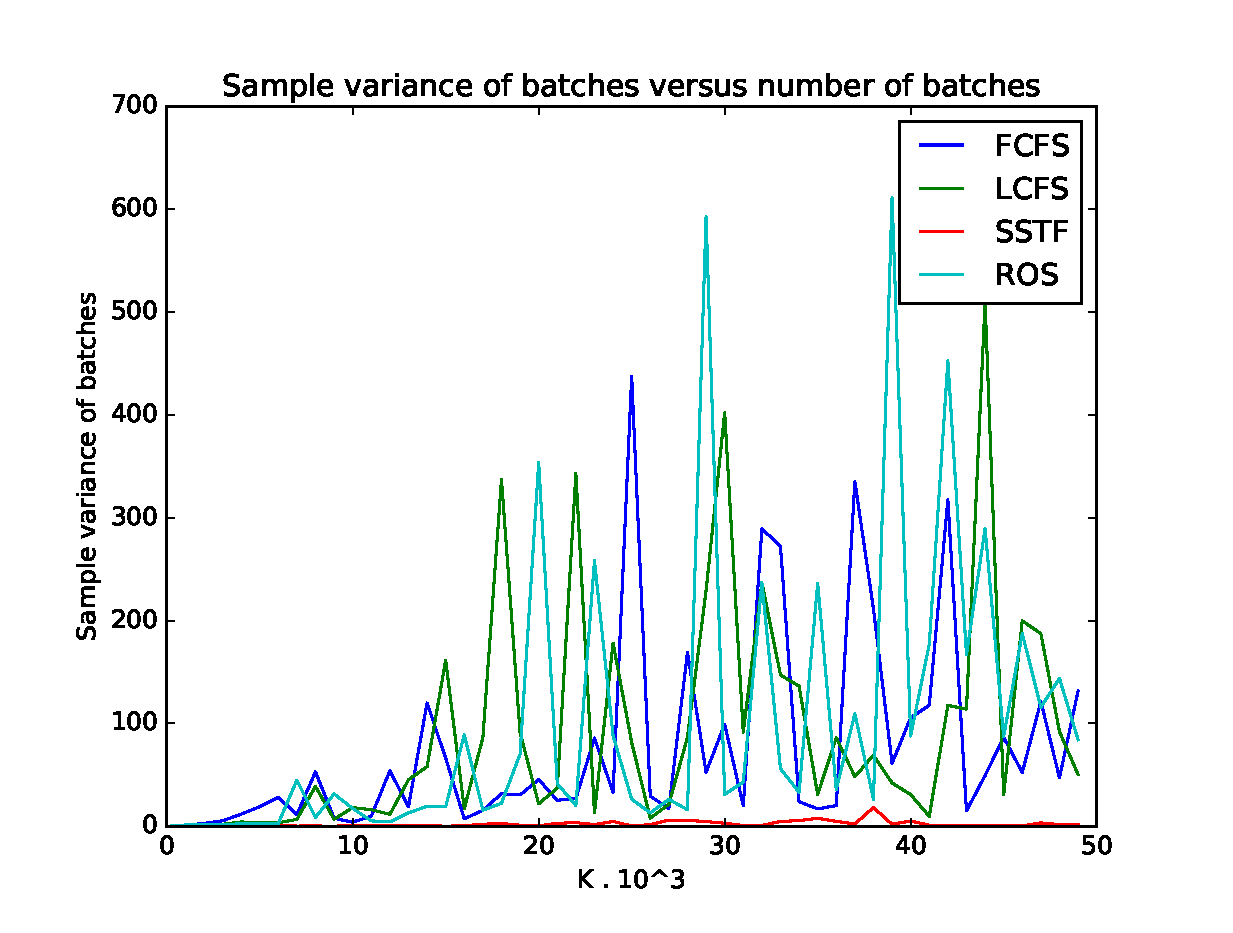
\includegraphics[width=0.6\linewidth]{../figures/batch_mean_var}
  \label{fig:bmv}
\end{figure}

\section{Code}
\label{sec:code}
\inputminted[numbersep=7pt,fontsize=\footnotesize,linenos]{python}{../src/main.py}
\captionof{listing}{main.py}
\inputminted[numbersep=7pt,fontsize=\footnotesize,linenos]{python}{../src/strategy.py}
\captionof{listing}{strategy.py}
\inputminted[numbersep=7pt,fontsize=\footnotesize,linenos]{python}{../src/agenda.py}
\captionof{listing}{agenda.py}
\inputminted[numbersep=7pt,fontsize=\footnotesize,linenos]{python}{../src/customer.py}
\captionof{listing}{customer.py}
\inputminted[numbersep=7pt,fontsize=\footnotesize,linenos]{python}{../src/FCFS.py}
\captionof{listing}{FCFS.py}
\inputminted[numbersep=7pt,fontsize=\footnotesize,linenos]{python}{../src/LCFS.py}
\captionof{listing}{LCFS.py}
\inputminted[numbersep=7pt,fontsize=\footnotesize,linenos]{python}{../src/SSTF.py}
\captionof{listing}{SSTF.py}
\inputminted[numbersep=7pt,fontsize=\footnotesize,linenos]{python}{../src/ROS.py}
\captionof{listing}{ROS.py}
\end{document}